\chapter{Исследовательская часть}
\section{Технические характеристики}
Технические характеристии устройства, на котором выполнялось тестирование:
\begin{itemize}
	\item Операционная система: Windows 10 Pro
	\item Память: 8 GiB
	\item Процессор: Intel(R) Core(TM) i5-8265U CPU @ 1.60GHz   1.80 GHz
\end{itemize}
Тестирование проводилось на ноутбуке, который был подключен к сети питания. Во время проведения тестирования ноутбук был нагружен только встроенными приложениями окружения, самим окружением и системой тестирования

\section{Временные харастеристики выполнения}
Замер процессорного времени работы алгоритмов производилось при помощи модуля time функцией process\_time().

Проведем анализ времени работы алгоритмов. Исходными данными будут случайно сгенерированные строки длиной {3, 4, 5, 6, 7, 8}. Единичные замеры выдадут крайне маленький результат, поэтому  проведем работу каждого алгоритма n = 1000 раз и поделим на число n. Получим среднее значение работы каждого из алгоритмов. Результат приведен на рис \ref{fg:ref1}:

\begin{figure}[ht!]
	\centering{
		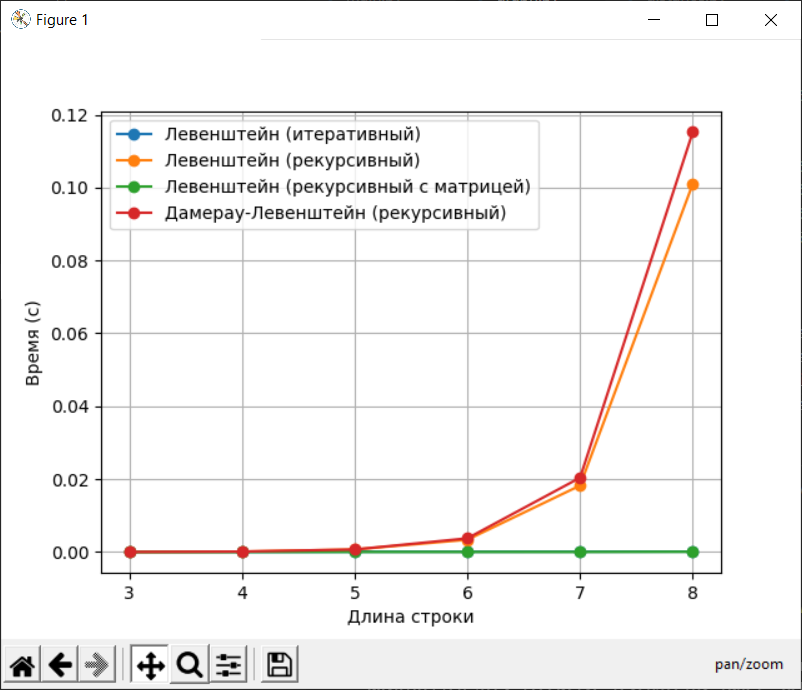
\includegraphics[width=10.6cm]{../../../../../../../msys64/home/Лев/bmstu_sem_5_aa/lab_01/report/image/graph}
		\caption{Сравнение времени работы алгоритмов Левенштейна.}
		\label{fg:ref1}}
\end{figure} 

Как видно из результатов, рекурсивный алгоритм Левенштейна без кэша и алгоритм Дамерау-Левенштейн имеют большой асимпотический рост, начиная уже со строки длиной 7. Последний имеет наибольший рост. Это объясняется тем, что этот алгоритм задействует дополнительную операцию - транспонирование, которая тоже приводит к вызову рекурсии. \\
Выполнив анализ двух остальных алгоритмов на значения входных строк длиной {25, 50, 75, 100, 125, 150}, получим слежующий результат, представленный на рис \ref{fg:ref2}:
\begin{figure}[ht!]
	\centering{
		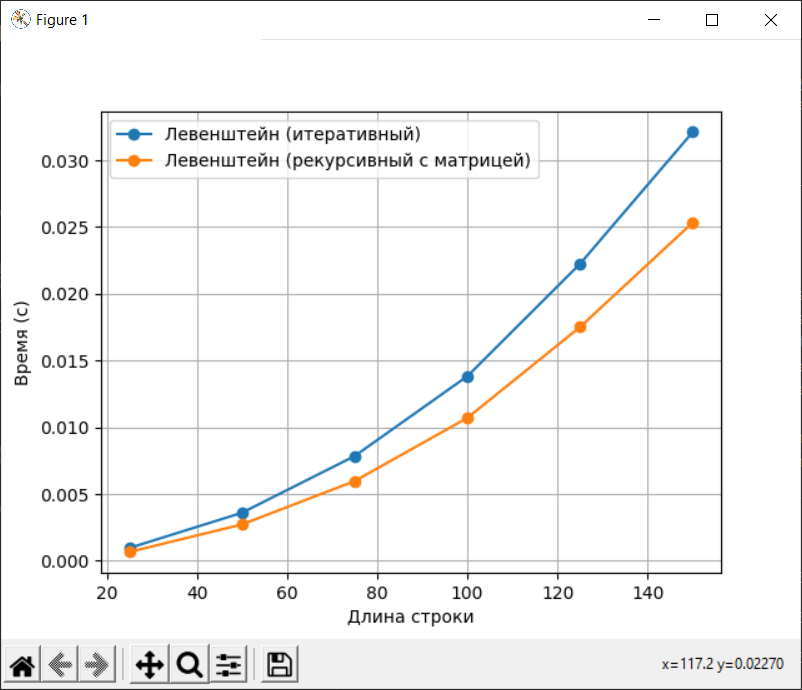
\includegraphics[width=10.6cm]{../../../../../../../msys64/home/Лев/bmstu_sem_5_aa/lab_01/report/image/graph_2}
		\caption{Сравнение времени работы рекурсивного и некурсивного алгоритмов Левенштейна.}
		\label{fg:ref2}}
\end{figure} 

Рекурсивный алгоритм Левенштейна с использованием матрицы выполняется быстрее, нежели чем итеративный с использованием двух строк. Это объясняется тем, что в итеративном случае выполняется дополнительная операция по обмену значений двух строк. На это необходимо дополнительное время.

\section{Объем потребляемой памяти}
Замеры используемой памяти и число вызовов рекурсии проводились при помощи модуля memory\_profiler. При исходных строках, длинною 3, требуется 52,8 Mb памяти. Результаты вызовов и объем потребляемой памяти приведены в таблице (4.3.1):
\begin{table}[ht!]
	\centering
	\captionsetup{singlelinecheck = false, justification=raggedleft}
	\caption{Число вызовов каждого алгоритма}
	\label{table:ref2}
	\begin{tabular}{|c|c|c|c|}
		\hline
		\multicolumn{3}{|c|}{Левенштейн} & Дамерау-Левенштейн \\ \cline{1-3} 
		\hline
		\multirow{2}{*}{Итеративный} &\multirow{2}{*}{Рекурсивный} & \multirow{2}{*}{Рекурсивный} & \multirow{2}{*}{Рекурсивный} \\
		с двумя строками & без кэша  & с матрицей & \\
		\hline
		1 & 94 & 28 & 94 \\ 
		\hline
	\end{tabular}
\end{table}\\
\\
Общее значение потребляемой памяти складывается по формуле \ref{eq:2}:
$$
S = n\_calls * V
\label{eq:2}
\eqno(4.3.1)
$$
где:
\begin{itemize}
	\item n\_calls - число вызовов функций
	\item V - объем памяти, занимаемый одним вызовом функции
\end{itemize}
По результатам исследования памяти алгоритм Левенштейна и Дамерау-Левенштейна потребляют больше всего памяти при работе. Итеративный алгоритм Левенштейна с двумя строками занимает меньше всего памяти

\section*{Вывод}
Характеристики алгоритмов, приведенные в разделах (4.2) и (4.3) позволяют сделать вывод о том, что рекурсивный вызов Левенштейна без кэша и Дамерау-Лвенштейна проигрывают как по скорости, так и по памяти итеративному. Причем рекурсивный алгоритм Левенштейна с матрицей работает быстрее, чем итеративный с двумя строками, но также проигрывает ему по памяти.

Сравнивая между собой рекурсивные вызовы алгоритмов Левенштейна и Дамерау-Левенштейна, можно сделать вывод о том, что рекурретный алгоритм поиска расстояния Левенштейна с матрицей выигрывает как по времени, так и по памяти, а рекуррентный Дамерау-Левенштейн проигрывает по обоим параметрам. Однако, стоит отметить, что в системах автоматического исправления текста, где чаще всего встречаются ошибки, связанные с транспозицией двух символов, алгоритм Дамерау-Левенштейна будет наиболее оптимальным.\\